\clearpage
\twocolumn[{%
\rqparent
\subsection{Design decisions}
\label{app:rq05_design_decisions}

\noindent\begin{minipage}[t]{0.485\textwidth}
\vspace{0pt}
\paragraph{Research Question.} \emph{At a given number of languages K, when does a small model rank a design choice (depth, data scheme, temperature, activation, optimizer) the way the 1.7B reference does, and how does the answer change with K?}

\paragraph{Setup.} We measure decision accuracy on six single-axis design decisions, each against the baseline (deep, scheme A, T = 1): depth (deep vs shallow at one nominal size, size-matched except at 600M, where shallow has 3.7 \% more non-embedding parameters), data scheme A vs B, data scheme A vs C, sampling temperature T = 1 vs T = 3, activation (xIELU vs SwiGLU) and optimizer (AdEMAMix vs Muon). The optimizer decision has no 1.7B evaluation yet, so it has no DA-size, DA-ckpt or effect at the reference on BPB or benchmarks. We read each decision on the seed-1904 runs of every ladder and data build (the replicate seeds only set the seed noise of the effect sizes). We read each decision per language setting K and then average over K. We read each decision on the per-language BPB of the languages that both levels train, and on the benchmark tasks: the accuracy tasks above chance at both the proxy and 1.7B, and their bBPB twins, which have no chance level and are about half to four fifths of the benchmark items. DA-size compares the final checkpoint of each proxy, 90M--1B, with the final checkpoint of the 1.7B run. DA-ckpt compares the earlier checkpoints of the 1.7B run with its final checkpoint.
\end{minipage}\hfill
\begin{minipage}[t]{0.485\textwidth}
\vspace{0pt}
\begin{rqfinding}
\textbf{1. Per-language BPB reads the temperature and list decisions at every proxy size, but the gated benchmarks almost never do.} On the BPB of the trained languages, temperature is read at 0.95--0.99 (mean over K15--K50) and the language lists at 0.77--1.00 (K8--K30). On the benchmarks every intervention sits at 0.45--0.63, and only the two K1 English-data swaps come near 0.75 (DCLMP 0.52--0.79, with 0.79 at 350M, and FWEB 0.57--0.75, with 0.75 at 600M). (Figure~\ref{fig:app_rq05_design_decisions}.)
\\
\\
\textbf{2. Per-language BPB reads temperature and the language lists in almost every cell.} Every proxy reads the temperature decision at 0.87--1.00 at every K, and the language-list decision at 0.83--1.00 in every cell except 1B at K30 (0.31).
\\
\\
\textbf{3. The depth decision on per-language BPB collapses at 350M and 600M.} It is 0.00 for 600M at all four K (the 600M depth pairs are not size-matched) and 0.00--0.97 for 350M, while 90M, 175M and 1B read it at 0.78--1.00.
\end{rqfinding}
\end{minipage}

\vspace{\baselineskip}
\noindent\begin{minipage}{\textwidth}
\centering
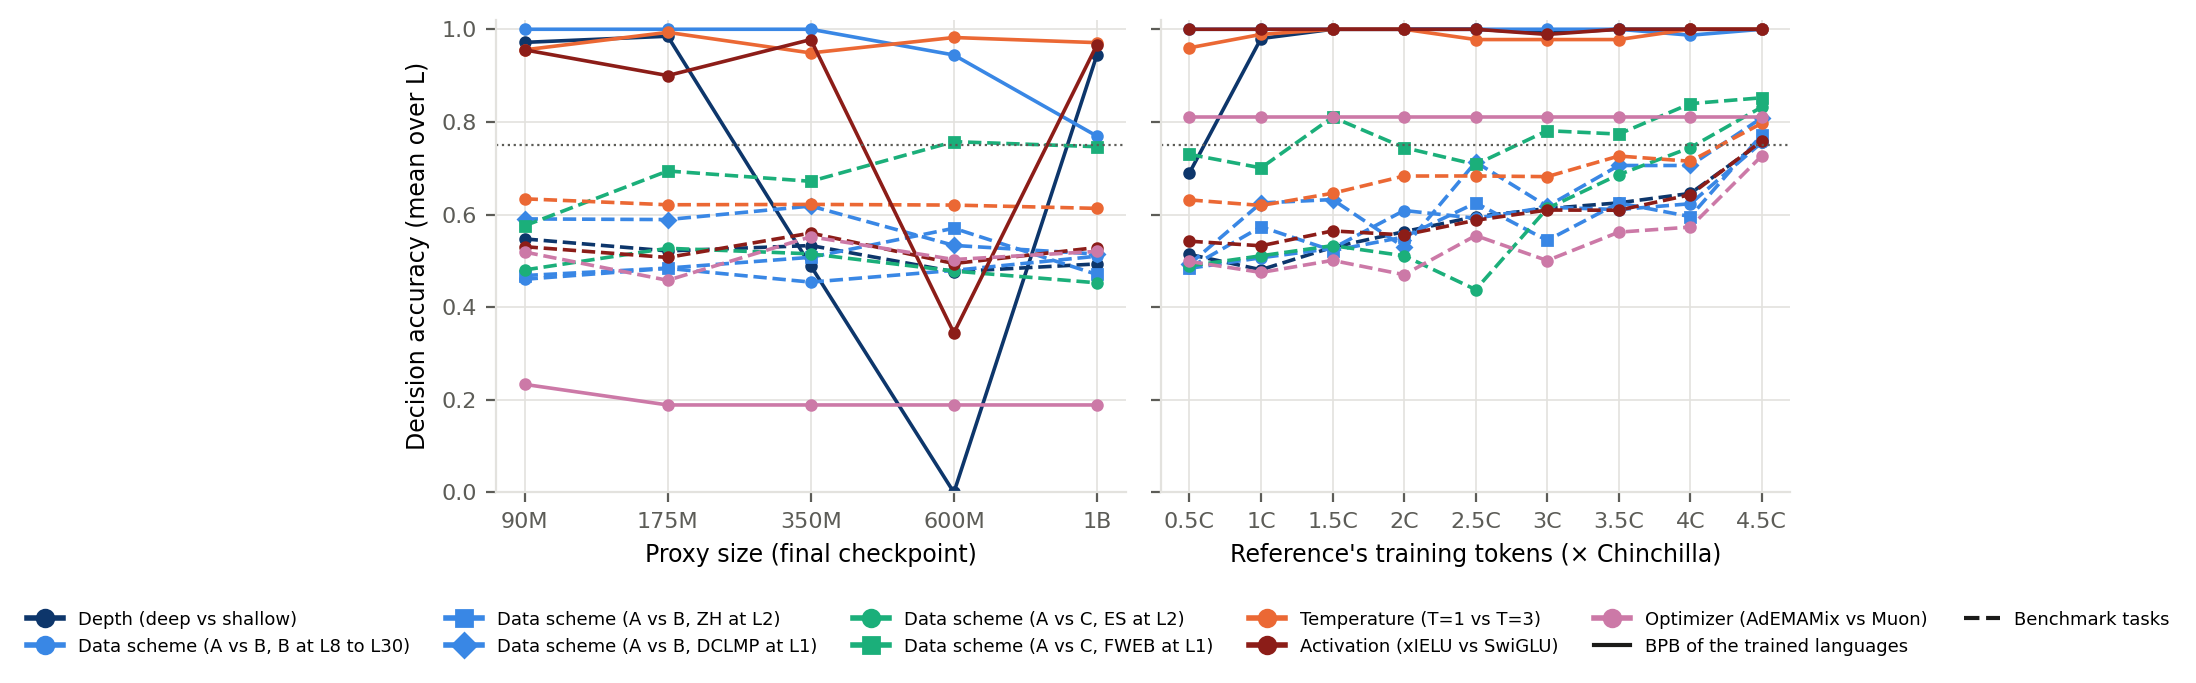
\includegraphics[width=\textwidth,height=0.36\textheight,keepaspectratio]{figures/app_rq05_design_decisions.png}
% source: src/signal-and-noise/analysis/rq05_design_decisions/pretraining/predictivity_seeds/da_all_lines_mono_axis_paper.png
\captionof{figure}{\textbf{Per-language BPB reads the temperature and list decisions at every proxy size, but the gated benchmarks almost never do.} Decision accuracy (mean over K) of each single-axis design decision. Left: the final checkpoint of each proxy size against the 1.7B final checkpoint (DA-size). Right: the earlier checkpoints of the 1.7B run against its final checkpoint (DA-ckpt), in Chinchilla multiples. Solid lines read the decision on the bits per byte of the trained languages and dashed lines on the benchmark tasks above chance. The dotted line marks 0.75.}
\label{fig:app_rq05_design_decisions}
\end{minipage}
}]
